% *********************************************************************
% © 2010–2021 Jeremy Sylvestre
%
% Permission is granted to copy, distribute and/or modify this document
% under the terms of the GNU Free Documentation License, Version 1.3 or
% any later version published by the Free Software Foundation; with no
% Invariant Sections, no Front-Cover Texts, and no Back-Cover Texts. A
% copy of the license is included in the appendix entitled “GNU Free
% Documentation License” that appears in the output document of this
% PreTeXt source code. All trademarks™ are the registered® marks of
% their respective owners.
%
% *********************************************************************

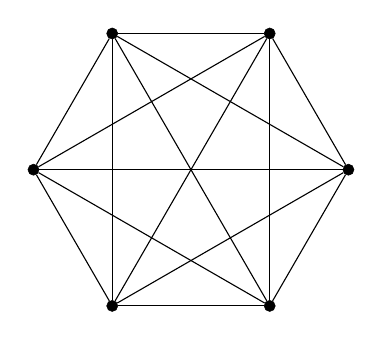
\begin{tikzpicture}[
	vertex/.style={ circle, draw, very thin, fill, inner sep=0pt, minimum size=4pt },
	vertexg/.style={ black!40!white, circle, draw, very thin, fill, inner sep=0pt, minimum size=4pt },
	vertexo/.style={ circle, draw, very thin, inner sep=0pt, minimum size=4pt }
]

\node[vertex] at (1,0) (k6v1) {};
\node[vertex] at (3,0) (k6v2) {};
\node[vertex] at (4,1.73) (k6v3) {};
\node[vertex] at (3,3.46) (k6v4) {};
\node[vertex] at (1,3.46) (k6v5) {};
\node[vertex] at (0,1.73) (k6v6) {};

\foreach \p in {k6v2,k6v3,k6v4,k6v5,k6v6} \draw (k6v1) to (\p);
\foreach \p in {k6v3,k6v4,k6v5,k6v6} \draw (k6v2) to (\p);
\foreach \p in {k6v4,k6v5,k6v6} \draw (k6v3) to (\p);
\foreach \p in {k6v5,k6v6} \draw (k6v4) to (\p);
\draw (k6v5) to (k6v6);

\end{tikzpicture}
